\documentclass[11pt]{article}
%\usepackage[14pt]{extsizes} % для того чтобы задать нестандартный 14-ый размер шрифта
%\usepackage[utf8]{inputenc}
\usepackage{mathtext}
\usepackage[english, russian]{babel}
\usepackage{amsmath}
\usepackage{amsfonts}
\usepackage{float}
\usepackage[margin=0.8in]{geometry}
\usepackage{multirow}
\usepackage{graphicx}
\usepackage[utf8x]{inputenc} % указать кодировку русского текста
\usepackage{fancyhdr}
\usepackage{indentfirst} % отступ в первой строке абзаца
\usepackage{wrapfig}
\usepackage{placeins}
\usepackage{caption}
\usepackage{amssymb}
\usepackage{mathtools}
\usepackage[thinc]{esdiff}
\usepackage{cmap}
\usepackage[table,xcdraw]{xcolor}
\usepackage{amsmath,amsfonts,amssymb,amsthm,mathtools, mathrsfs}
\usepackage{breqn}
\usepackage{subcaption}

\pagestyle{fancy}
\begin{document}
\begin{titlepage}
\begin{center}
%\vspace*{1cm}
\large{\small ФЕДЕРАЛЬНОЕ ГОСУДАРСТВЕННОЕ АВТОНОМНОЕ ОБРАЗОВАТЕЛЬНОЕ\\ УЧРЕЖДЕНИЕ ВЫСШЕГО ОБРАЗОВАНИЯ\\ МОСКОВСКИЙ ФИЗИКО-ТЕХНИЧЕСКИЙ ИНСТИТУТ\\ (НАЦИОНАЛЬНЫЙ ИССЛЕДОВАТЕЛЬСКИЙ УНИВЕРСИТЕТ)\\ ФИЗТЕХ-ШКОЛА РАДИОТЕХНИКИ И КОМПЬЮТЕРНЫХ ТЕХНОЛОГИЙ}
\vfill
\line(1,0){430}\\[1mm]
\huge{Лабораторная работа 3.7.1}\\
\huge\textbf{Скин-эффект в полом цилиндре.}\\
\line(1,0){430}\\[1mm]
\vfill
\begin{flushright}
\normalsize{Устюжанина Мария}\\
\normalsize{\textbf{Группа Б01-107}}\\
\end{flushright}
\end{center}
\end{titlepage}
\fancyhead[L] {Работа 3.7.1}

\par \textbf{Цель работы:} исследование проникновения переменного магнитного поля в медный полый цилиндр.

\par \textbf{В работе используются:} генератор звуковой частоты, соленоид, намотанный на полый цилиндрический каркас из диэлектрика, медный экран в виде трубки, измерительная катушка, амперметр, вольтметр, осциллограф.

\section{Экспериментальная установка}
    \begin{figure}[H]
    \center{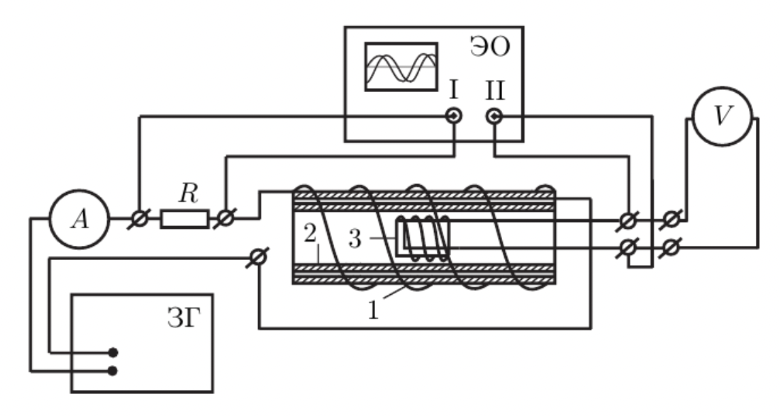
\includegraphics[scale=0.7]{ustanovka.png}}
    \caption{Схема экспериментальной установки.}
    \label{pic:3}
    \end{figure}
\newpage

\subsection{Подготовка}
Приняв проводимость меди для оценки равной \( \sigma = 5\cdot 10^{7}\; См/м \) расчитаем частоту \( \nu_h\; Гц \),
при которой толщина стенок экрана равна скиновой длине \( \delta = h = 1.5\; mm \). По формуле:
\[ \delta = \sqrt{\frac{2}{\omega \sigma \mu_0}} \Rightarrow \nu_h = \frac{1}{\pi\sigma\mu_0 h^2} = 2250\; Гц \]
\subsection{Измерения в диапазоне \((0.01мкГн - 0.05мкГн)\)}
Получим знависимость соотношения \( \xi = U/(\nu I) \) от частоты \(\nu\):
\begin{table}[H]
    \centering
    \begin{tabular}{|c|c|c|c|}
    \hline
    \(\nu\), Гц & U, В  & I, A  & \(\xi = U/(\nu I)\) \\\hline
    22.5 & 0.195 & 0.461 & 0.0188   \\\hline
    31.5 & 0.269 & 0.457 & 0.0187   \\\hline
    40.5 & 0.338 & 0.453 & 0.0184   \\\hline
    49.5 & 0.403 & 0.448 & 0.0182   \\\hline
    58.5 & 0.463 & 0.442 & 0.0179   \\\hline
    67.5 & 0.518 & 0.436 & 0.0176   \\\hline
    76.5 & 0.569 & 0.43  & 0.0173   \\\hline
    85.5 & 0.614 & 0.423 & 0.0170   \\\hline
    94.5 & 0.654 & 0.418 & 0.0166   \\\hline
    103.5& 0.69  & 0.412 & 0.0162   \\\hline
    112.5& 0.723 & 0.406 & 0.0158   \\\hline
    \end{tabular}
\end{table}

\begin{figure}[H]
    \centering
    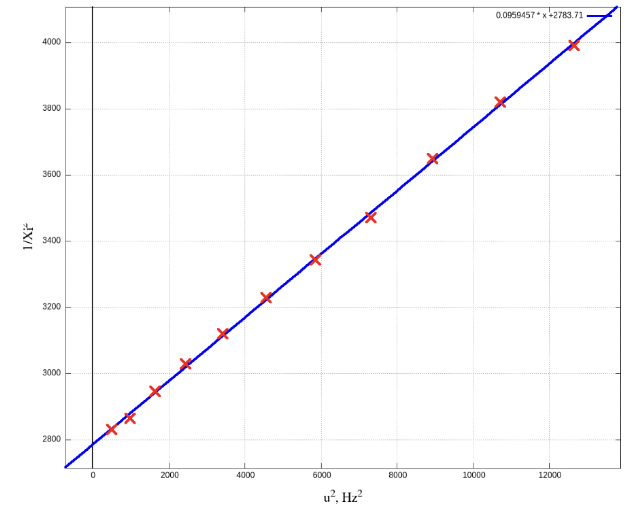
\includegraphics[width=0.8\textwidth]{1.png}
    \caption{график \( 1/\xi^2(\nu^2) \)}
    \label{plot1}
\end{figure}

Получена зависимость вида \( 1/\xi^2 = a\cdot \nu^2 + b \):
\[ a = (0.096 \pm 7\cdot10^{-4}) \]
\[ b = (2783 \pm 2.7) \]
\subsection{Измерения в диапазоне \((0.05мкГн - 0.5мкГн)\)}
Исследуем зависимости \(\xi\) и \(\psi\) от \(\nu\):
\begin{table}[H]
    \centering
    \begin{tabular}{|c|c|c|c|c|}
    \hline
    \(\nu\), Гц & U, В  & I, A  & \(\psi\), рад & \(\xi = U/(\nu I)\) \\\hline
    112.5   & 0.721 & 0.404 & 3.70 & 0.0159\\\hline
    128.5   & 0.769 & 0.394 & 3.87 & 0.0152\\\hline
    144.5   & 0.809 & 0.386 & 4.06 & 0.0145\\\hline
    160.5   & 0.841 & 0.378 & 4.05 & 0.0139\\\hline
    176.5   & 0.868 & 0.371 & 4.04 & 0.0133\\\hline
    192.5   & 0.89  & 0.366 & 4.11 & 0.0126\\\hline
    208.5   & 0.908 & 0.361 & 4.06 & 0.0121\\\hline
    225     & 0.923 & 0.356 & 4.05 & 0.0115\\\hline
    315     & 0.967 & 0.338 & 4.32 & 0.0091\\\hline
    405     & 0.98  & 0.327 & 4.27 & 0.0074\\\hline
    495     & 0.979 & 0.318 & 4.29 & 0.0062\\\hline
    585     & 0.971 & 0.311 & 4.43 & 0.0053\\\hline
    675     & 0.959 & 0.304 & 4.61 & 0.0047\\\hline
    765     & 0.943 & 0.297 & 4.59 & 0.0042\\\hline
    855     & 0.927 & 0.291 & 4.68 & 0.0037\\\hline
    945     & 0.908 & 0.284 & 4.62 & 0.0034\\\hline
    1035    & 0.888 & 0.278 & 4.71 & 0.0031\\\hline
    \end{tabular}
\end{table}

\begin{figure}[H]
    \centering
    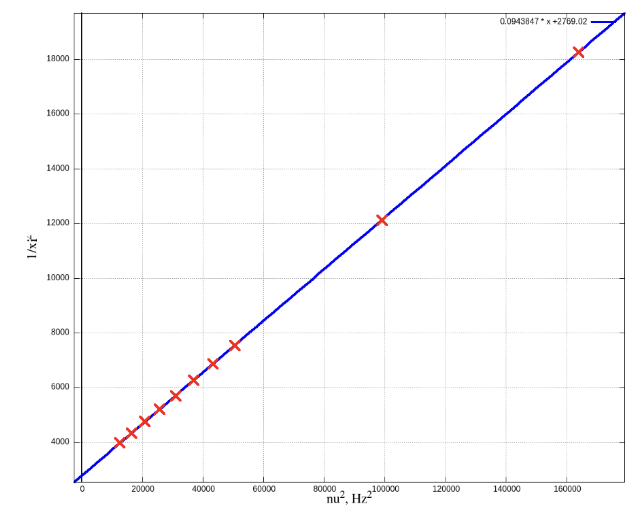
\includegraphics[width=0.8\textwidth]{2.png}
    \caption{график \( 1/\xi^2(\nu^2) \)}
    \label{plot2}
\end{figure}

Получена зависимость вида \( 1/\xi^2 = a\cdot \nu^2 + b \):
\[ a = (0.094 \pm 8\cdot10^{-5}) \]
\[ b = (2769 \pm 3.5) \]

Что совпадает со значениями на интервале \((0.01мкГн - 0.05мкГн)\), говоря о том, 
что зависимость одинаковая на обоих диапазонах

\begin{figure}[H]
    \centering
    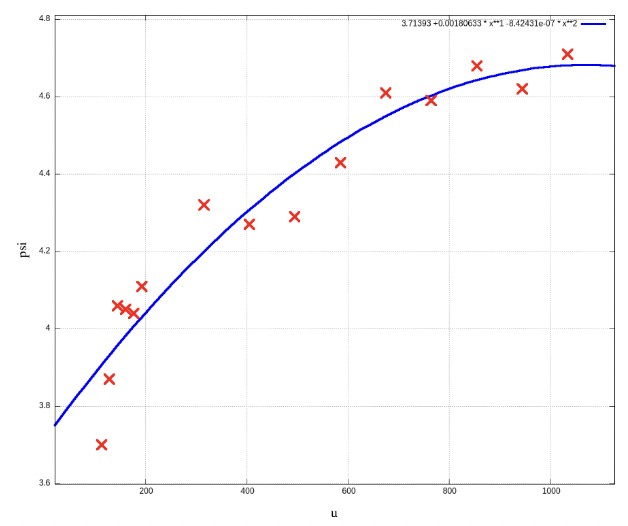
\includegraphics[width=0.8\textwidth]{3.png}
    \caption{график \( \psi(\nu) \)}
\end{figure}

Аппроксимируем многочленом 2 степени:
\[ \psi = 3.7 + 0.002\nu -8.4\cdot 10^{-7}\nu^2\; рад \]

\subsection{Измерения в диапазоне \((0.5мкГн - 15мкГн)\)}
Исследуем зависимости \(\xi\) и \(\psi\) от \(\nu\):
\begin{table}[H]
    \centering
    \begin{tabular}{|c|c|c|c|c|}
    \hline
    \(\nu\), Гц & U, В  & I, A  & \(\psi\), рад & \(\xi = U/(\nu I)\) \\\hline
    1125  & 0.867 & 0.271 & 4.71 & 0.00284 \\\hline
    3330  & 0.468 & 0.148 & 5.02 & 0.0009  \\\hline
    5535  & 0.288 & 0.095 & 5.41 & 0.00055 \\\hline
    7740  & 0.197 & 0.068 & 5.80 & 0.0004  \\\hline
    9945  & 0.143 & 0.053 & 6.03 & 0.0003  \\\hline
    12150 & 0.106 & 0.041 & 6.13 & 0.00021 \\\hline
    14355 & 0.081 & 0.034 & 6.28 & 0.00017 \\\hline
    16560 & 0.062 & 0.028 & 6.70 & 0.00013 \\\hline
    18765 & 0.049 & 0.023 & 6.75 & 0.00011 \\\hline
    20970 & 0.039 & 0.019 & 7.07 & 9.8E-05 \\\hline
    23175 & 0.031 & 0.015 & 7.14 & 8.9E-05 \\\hline
    25380 & 0.026 & 0.012 & 4.55 & 8.5E-05 \\\hline
    27585 & 0.023 & 0.008 & 8.37 & 0.00010 \\\hline
    29790 & 0.022 & 0.006 & 8.50 & 0.00012 \\\hline
    31995 & 0.023 & 0.003 & 9.22 & 0.00024 \\\hline
    \end{tabular}
\end{table}

Аппроксимируем многочленом 2 степени:
\[ \xi = 21.4 - 0.0023\nu + 5.6\cdot 10^{-8}\nu^2 \]

\begin{figure}[H]
    \centering
    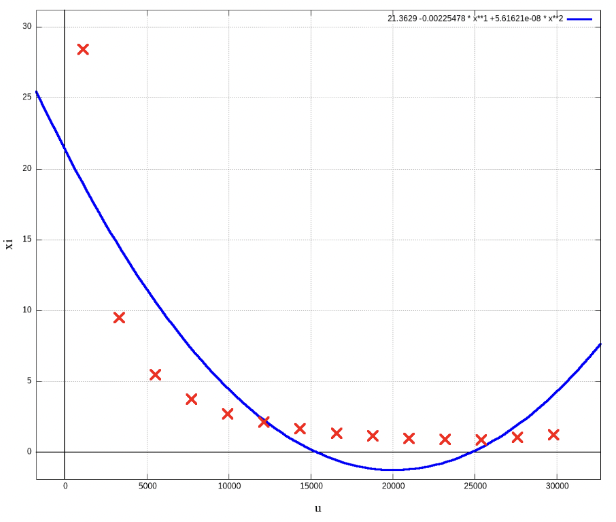
\includegraphics[width=0.8\textwidth]{4.png}
    \caption{график \( \xi(\nu) \)}
\end{figure}

Аппроксимируем прямой вида \( \psi = a\nu + b \) :
\[ a = 1.3\cdot 10^{-4} \pm 6.3\cdot 10^{-6} \]
\[ b = 4.55 \pm 0.06 \]

\begin{figure}[H]
    \centering
    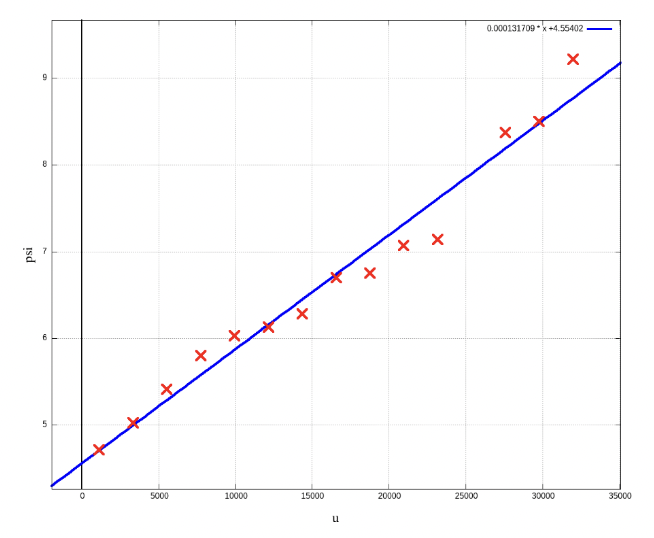
\includegraphics[width=0.8\textwidth]{5.png}
    \caption{график \( \psi(\nu) \)}
\end{figure}

\subsection{Зависимость \(L\) от \(\nu\)}

\begin{table}[H]
    \centering
    \begin{tabular}{|c|c|}
    \hline
    \(\nu\), Гц & \(L\), \(\mu H\) \\\hline
    40  & 550 \\\hline
    400 & 4300\\\hline
    750 & 3400\\\hline
    1000& 3200\\\hline
    1500& 3100\\\hline
    2000& 3060\\\hline
    2500& 3050\\\hline
    \end{tabular}
\end{table}

Аппроксимируем многочленом 2 степени:
\[ L = 4885 - 2.1\nu + 0.0006\nu^2 \]


\begin{figure}[H]
    \centering
    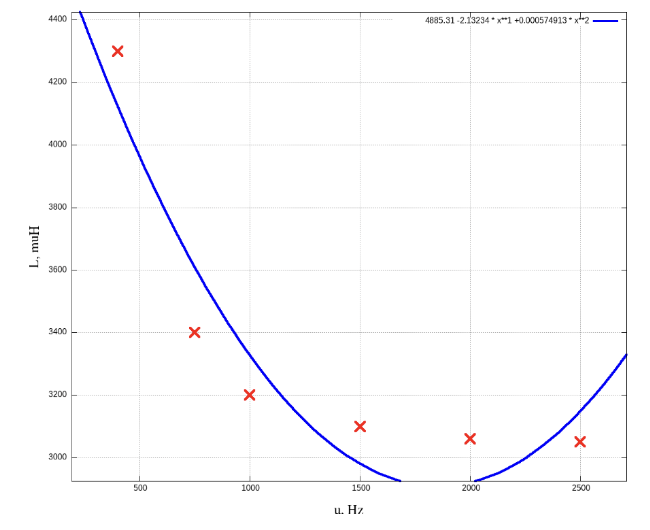
\includegraphics[width=0.8\textwidth]{6.png}
    \caption{график \( L(\nu) \)}
    \label{fig:L}
\end{figure}

\section {Обработка экспериментальных данных}
\subsection{}
\label{sigma_1}
По графикам на рисунках \ref{plot1} и \ref{plot2} легко убедиться что зависимость \( 1/\xi^2(\nu^2) \)
имеет линейный вид.

Экстраполируя полученную зависимость к точке \( \nu = 0 \), соответствующей величине \( \frac{|H_1|}{|H_0|} = 1 \)
определим коэффициент пропорциональности \( \xi_0 \) между \( \xi \) и \( \frac{|H_1|}{|H_0|} \): 
\[ \xi_0 = 53 \]

Из того что в области низких частот
\[ \left(\frac{|H_1|}{|H_0|}\right)^2 = (\xi_0\xi)^2 \simeq \frac{1}{1 + A\nu^2} \]
получим что угловой коэффициент зависимости \( 1/\xi^2(\nu^2) \) равен
\[ k = \pi ah\mu_0\xi_0\sigma = (0.096 \pm 7\cdot10^{-4}) \]
Отсюда найдём првоводимость меди:
\[ \sigma = \frac{k}{\pi ah\mu_0\xi_0} = 13.6\; \frac{MСм}{м} \]

\subsection{}\label{sigma_2}
Перерисуя график \( \psi \) от \( \nu \) и опроксимируя прямой получим:

\begin{figure}[H]
    \centering
    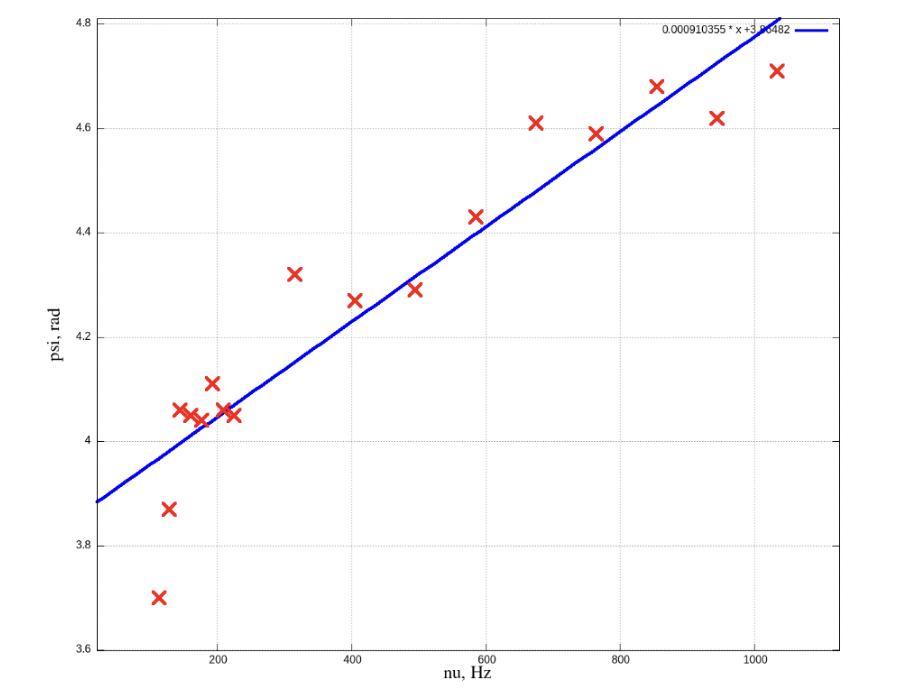
\includegraphics[width=0.8\textwidth]  {psi.png}
    \caption{график \( \psi(\nu) \)}
\end{figure}

Полученная зависимость вида \( \psi = a\cdot\nu + b \)
\[ a = (9 \pm 0.08)\; 10^{-3} рад/Гц \]
\[ b = (3.9 \pm 0.02)\; рад \] 

Из того что 
\[ \tg(\psi) = \frac{ah}{\delta^2} \]
и
\[ \delta^2 = \sqrt{\frac{1}{\pi\nu\sigma\mu_0}} \]
получим:

\[ \tg(\psi) = \pi ah\sigma\mu_0\nu \]

И тогда через коэффицент пропорциональности в зависимости \( \psi(\nu) \) найдём проводимость меди:
\[ \sigma = \frac{\tg(\psi)/\nu}{\pi ah\mu_0} = 67.5\; \frac{MСм}{м} \]

\subsection{}\label{sigma_3}

Построим график зависимости \( \phi = \psi - \frac{\pi}{4} \) от \(\sqrt{\nu}\):

\begin{figure}[H]
    \centering
    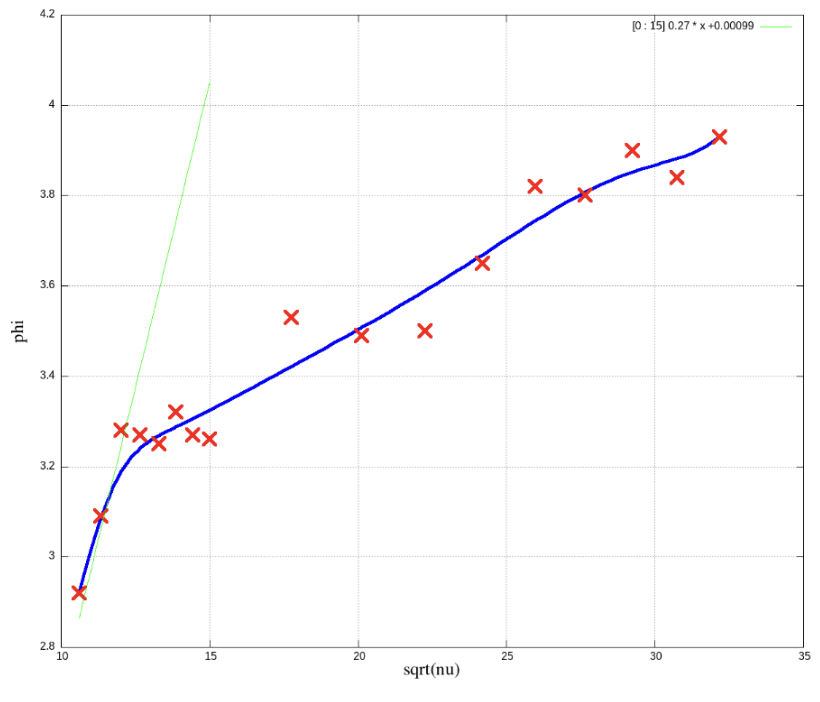
\includegraphics[width=0.8\textwidth]{phi.png}
    \caption{график \( \phi(\sqrt{\nu}) \)}
\end{figure}

Угловой коэффициент касательной:
\[ k = 0.27 \]

Отсюда, т.к.
\[ \psi = \frac{\pi}{4} + h\sqrt{\pi\nu\sigma\mu_0}\]
получим значение:
\[ \sigma = \frac{k^2}{h^2\pi\mu_0} = 8207\; \frac{МСм}{м}\]
Это значение не выглядит реалистичным, что можно связать с ошибками экспериментаторов во время
измерении разности фаз.

\subsection{} \label{sigma_4}
По результатам измерений, изображённым на Рис. \ref{fig:L} Определим максимальное и минимальное значение индуктивности:
\[ L_{min} = 550\; \mu H \]
\[ L_{max} = 3060\; \mu H \]

Построим график зависимости \( (L_{max} - L_{min})/(L - L_{min}) \) от \(\nu^2\) (\(10^6\; Гц^2\)):
\begin{figure}[H]
    \centering
    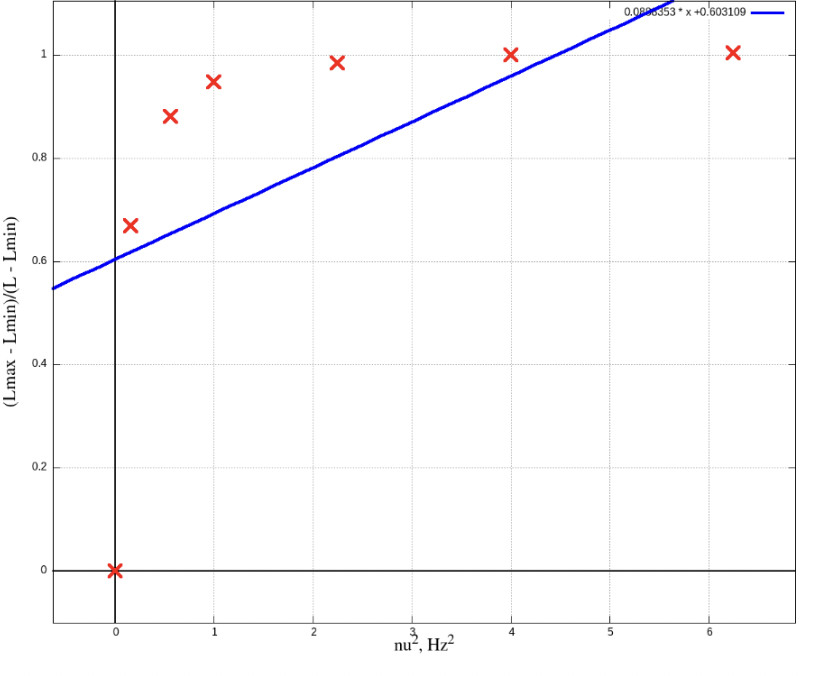
\includegraphics[width=0.8\textwidth]{L.png}
    \caption{график зависимости \( (L_{max} - L_{min})/(L - L_{min})\) от \(\nu^2 \cdot 10^6\; Гц^2\) \)}
\end{figure}

Из графика видно, что измерения плохо опроксимируются прямой. Скорее всего это произошло в виду
неправильного обращения экспериментаторов с измеряющим прибором и установкой. В следствии этого
оценить проводимость материала исходя из этого эксперимента не предоставляется возможным.

\subsection{}

Сравним значения проводимости медного экрана, полученные в ходе различных экспериментов:
\begin{table}[H]
    \centering
    \begin{tabular}{|c|c|c|c|c|}
        \hline
        \(\sigma\; 10^7 См/м\) из 3.1 & \(\sigma\; 10^7 См/м\) из 3.2  & \(\sigma\; 10^7 См/м\) из 3.3  & \(\sigma\; 10^7 См/м\) из 3.4&  \(\sigma\; 10^7 См/м\) табличное\\\hline
        1.36 & 6.75 & 820 & -- & 5.96  \\\hline
    \end{tabular}
\end{table}

Можно заметить, что значения полученные в пунктах 3.1 и 3.2 достаточно близки к табличному.
В то же время значение, полученное в пункте 3.3 далеко от табличного, а в 3.4 его вычисление
и вовсе не предоставляется возможным, что можно связать с ошибками экспериментаторов в ходе этих экспериментов.

\subsection{}
Расчитаем, используя значение \(\xi_0 = 53\), полученное в пункте 3.1, значение \(|H_1|/|H_0|\) для всех измерений.
Используем формулу
\[\frac{H_1}{H_0} = \xi\xi_0\]
(
Так же получим из формулы
\[ \frac{H_1}{H_0} = \frac{1}{\cosh(\alpha h) + \frac{1}{2}\alpha a\cdot\sinh(\alpha h)}, \]
где 
\[ \alpha = \sqrt{\2\pi\nu\sigma\mu}\cos(\pi/4) \]
а \(a\) и \(h\) - известные нам параметры установки, получим теоретические значения \(\frac{H_1}{H_0}\). 
Изобразим всё на графиках:

\begin{figure}[H]
    \centering
    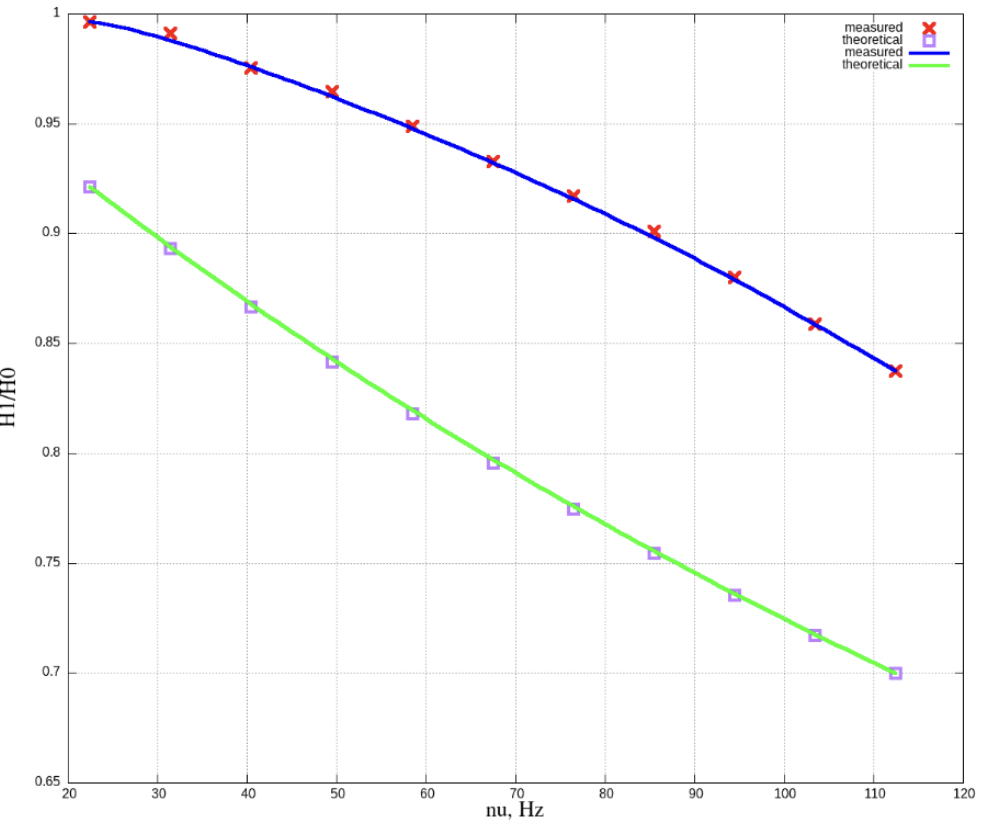
\includegraphics[width=1\textwidth]{H-low.png}
    \capture {Теоретический и экспериментальный графики зависимостей \(H_1/H_0\) от \(\nu\) для низких частот}
    \label{H-low}
\end{figure}

\begin{figure}[H]
    \centering
    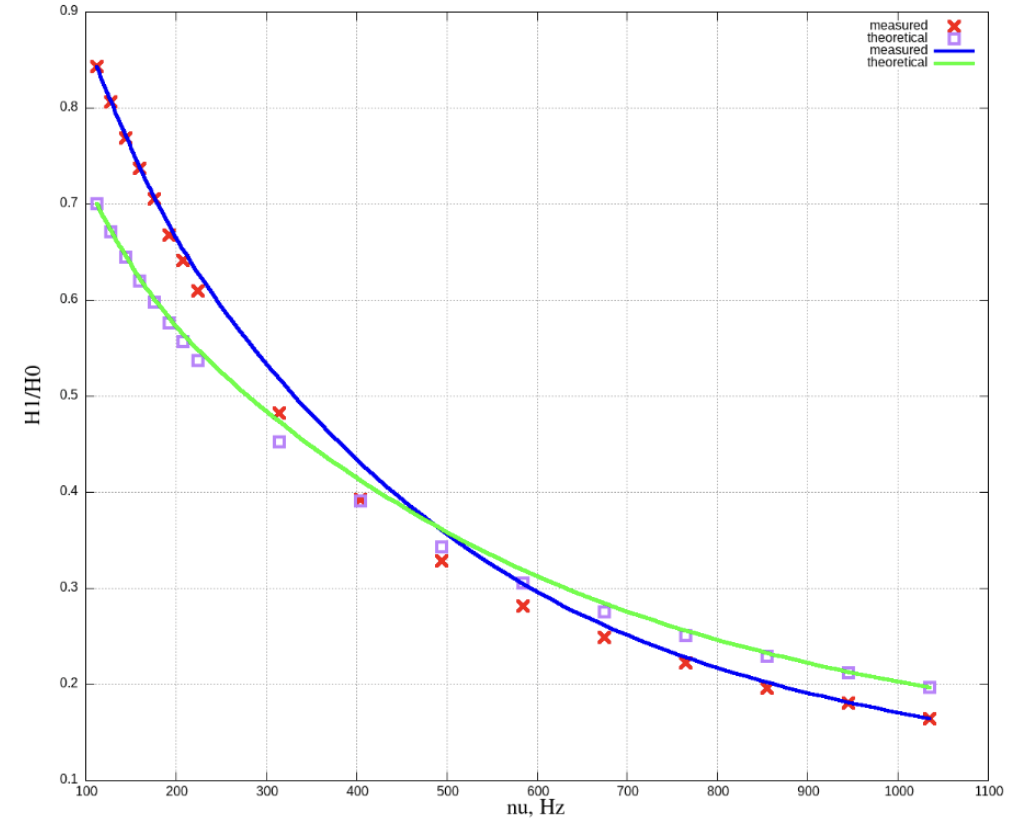
\includegraphics[width=1\textwidth]{H-mid.png}
    \capture {Теоретический и экспериментальный графики зависимостей \(H_1/H_0\) от \(\nu\) для средних частот}
    \label{H-mid}
\end{figure}

\begin{figure}[H]
    \centering
    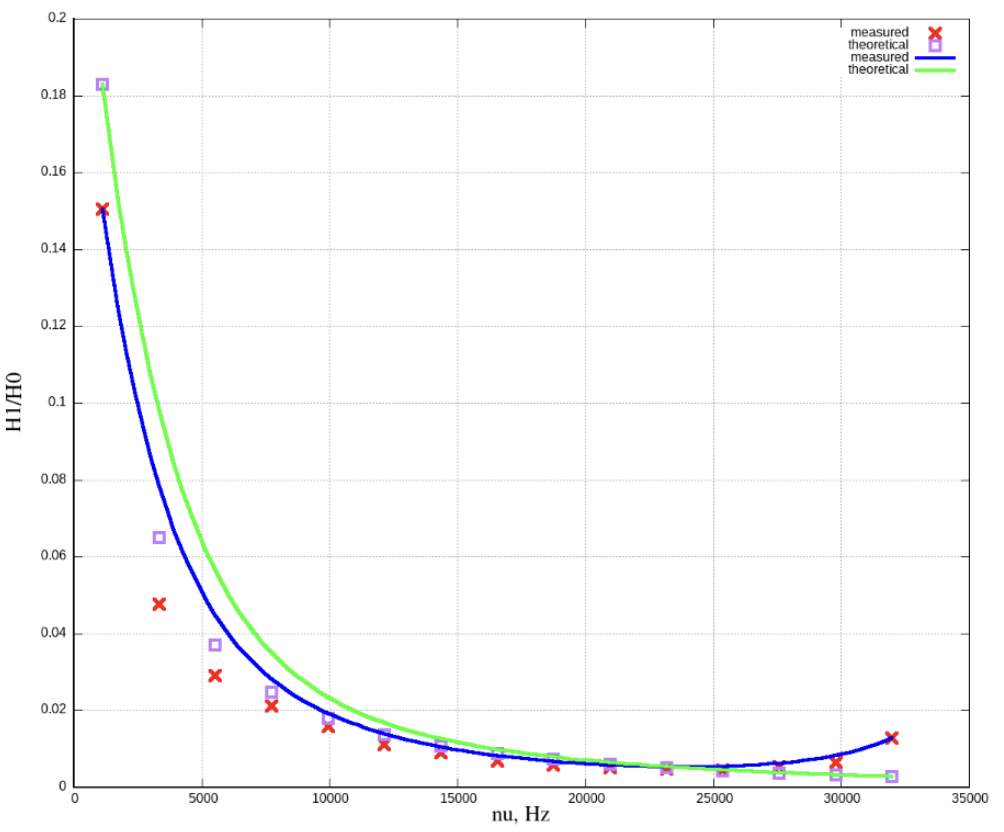
\includegraphics[width=1\textwidth]{H-hight.png}
    \capture {Теоретический и экспериментальный графики зависимостей \(H_1/H_0\) от \(\nu\) для высоких частот}
    \label{H-hight}
\end{figure}

Мы видим, что теоретические и экспериментальные значения \(H_1/H_0\) достаточно точно совпадают для всех диапазонов.
Наибольшее отличие заметно в области низких частот, что можно связать с недостаточной точностью вычислений или измерений в этом
диапазоне.


\section{Выводы}
Была проведена попытка измерения проводимости материала циллиндра 4 разными способами (теоретическое значение \( 5\cdot10^7\; \frac{См}{м} \)). Результаты:
\begin{enumerate}
    \item Из углового коэффициента зависимости \(1/\xi\) от \(\nu^2\). Получено значение \(1.36\cdot10^7\;\frac{См}{м}\). Это значение поп порядку
    совпадает с табличным.
    \item Из зависимости \( \tg(\psi) \) от \( \nu \). Получено значение \( 6.75\cdot10^7\; \frac{См}{м} \) . Это значение очень близко к табличному.
    \item Из угла наклона касательной к графику \( \psi \) от \(\sqrt{\nu}\) в области низких частот. Получено значение \( 821\cdot10^7\; \frac{См}{м} \),
    что отличается от табличного на несколько порядков.
    \item Из зависимости \( (L_{max} - L_{min})/(L - L_{min}) \) от \(\nu^2\). Попытка вычисления \(\sigma\) оказалась неудачной, т.к. измеренные значения
    нельзя хоть сколько-нибудь точно опроксимировать прямой.
\end{enumerate}
Можно сделать вывод, что только первые 2 способа измерения \(\sigma\) оказались удачными и дали правильные значения.

Были сравнены теоретически-вычисленное и измеренные значения отношения амплитуд магнитных полей для низких, средних и высоких частот.
Все сравнения показывают, что, хоть и в области низких частот значения незначительно отличались, тренд оказался одинаковым.

\section{Ход работы:}


\subsection{Подготовка}
Приняв проводимость меди для оценки равной \( \sigma = 5\cdot 10^{7}\; См/м \) расчитаем частоту \( \nu_h\; Гц \),
при которой толщина стенок экрана равна скиновой длине \( \delta = h = 1.5\; mm \). По формуле:
\[ \delta = \sqrt{\frac{2}{\omega \sigma \mu_0}} \Rightarrow \nu_h = \frac{1}{\pi\sigma\mu_0 h^2} = 2250\; Гц \]
\subsection{Измерения в диапазоне \((0.01мкГн - 0.05мкГн)\)}
Получим знависимость соотношения \( \xi = U/(\nu I) \) от частоты \(\nu\):
\begin{table}[H]
    \centering
    \begin{tabular}{|c|c|c|c|}
    \hline
    \(\nu\), Гц & U, В  & I, A  & \(\xi = U/(\nu I)\) \\\hline
    22.5 & 0.195 & 0.461 & 0.0188   \\\hline
    31.5 & 0.269 & 0.457 & 0.0187   \\\hline
    40.5 & 0.338 & 0.453 & 0.0184   \\\hline
    49.5 & 0.403 & 0.448 & 0.0182   \\\hline
    58.5 & 0.463 & 0.442 & 0.0179   \\\hline
    67.5 & 0.518 & 0.436 & 0.0176   \\\hline
    76.5 & 0.569 & 0.43  & 0.0173   \\\hline
    85.5 & 0.614 & 0.423 & 0.0170   \\\hline
    94.5 & 0.654 & 0.418 & 0.0166   \\\hline
    103.5& 0.69  & 0.412 & 0.0162   \\\hline
    112.5& 0.723 & 0.406 & 0.0158   \\\hline
    \end{tabular}
\end{table}

\begin{figure}[H]
    \centering
    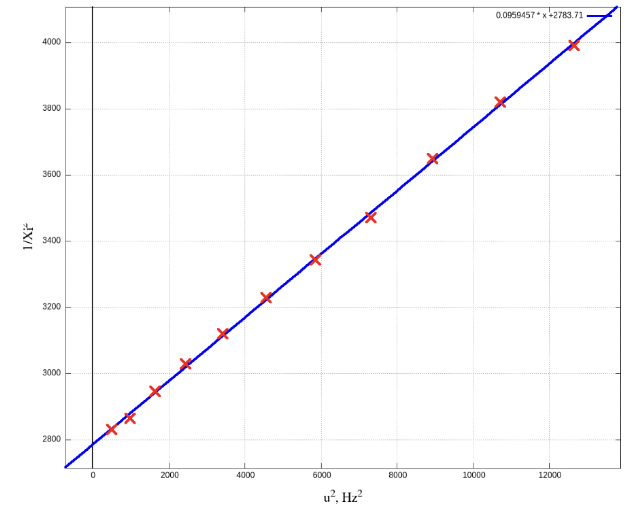
\includegraphics[width=0.8\textwidth]{1.png}
    \caption{график \( 1/\xi^2(\nu^2) \)}
    \label{plot1}
\end{figure}

Получена зависимость вида \( 1/\xi^2 = a\cdot \nu^2 + b \):
\[ a = (0.096 \pm 7\cdot10^{-4}) \]
\[ b = (2783 \pm 2.7) \]
\subsection{Измерения в диапазоне \((0.05мкГн - 0.5мкГн)\)}
Исследуем зависимости \(\xi\) и \(\psi\) от \(\nu\):
\begin{table}[H]
    \centering
    \begin{tabular}{|c|c|c|c|c|}
    \hline
    \(\nu\), Гц & U, В  & I, A  & \(\psi\), рад & \(\xi = U/(\nu I)\) \\\hline
    112.5   & 0.721 & 0.404 & 3.70 & 0.0159\\\hline
    128.5   & 0.769 & 0.394 & 3.87 & 0.0152\\\hline
    144.5   & 0.809 & 0.386 & 4.06 & 0.0145\\\hline
    160.5   & 0.841 & 0.378 & 4.05 & 0.0139\\\hline
    176.5   & 0.868 & 0.371 & 4.04 & 0.0133\\\hline
    192.5   & 0.89  & 0.366 & 4.11 & 0.0126\\\hline
    208.5   & 0.908 & 0.361 & 4.06 & 0.0121\\\hline
    225     & 0.923 & 0.356 & 4.05 & 0.0115\\\hline
    315     & 0.967 & 0.338 & 4.32 & 0.0091\\\hline
    405     & 0.98  & 0.327 & 4.27 & 0.0074\\\hline
    495     & 0.979 & 0.318 & 4.29 & 0.0062\\\hline
    585     & 0.971 & 0.311 & 4.43 & 0.0053\\\hline
    675     & 0.959 & 0.304 & 4.61 & 0.0047\\\hline
    765     & 0.943 & 0.297 & 4.59 & 0.0042\\\hline
    855     & 0.927 & 0.291 & 4.68 & 0.0037\\\hline
    945     & 0.908 & 0.284 & 4.62 & 0.0034\\\hline
    1035    & 0.888 & 0.278 & 4.71 & 0.0031\\\hline
    \end{tabular}
\end{table}

\begin{figure}[H]
    \centering
    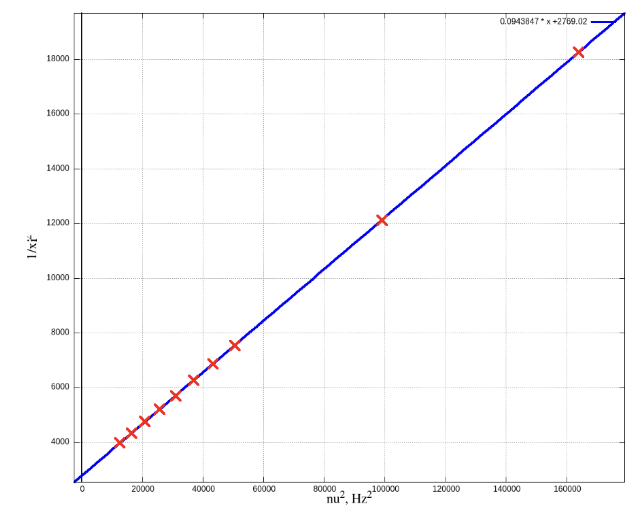
\includegraphics[width=0.8\textwidth]{2.png}
    \caption{график \( 1/\xi^2(\nu^2) \)}
    \label{plot2}
\end{figure}

Получена зависимость вида \( 1/\xi^2 = a\cdot \nu^2 + b \):
\[ a = (0.094 \pm 8\cdot10^{-5}) \]
\[ b = (2769 \pm 3.5) \]

Что совпадает со значениями на интервале \((0.01мкГн - 0.05мкГн)\), говоря о том, 
что зависимость одинаковая на обоих диапазонах

\begin{figure}[H]
    \centering
    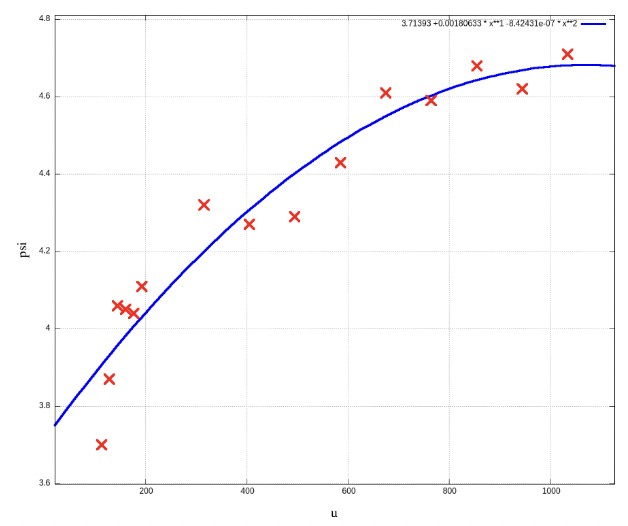
\includegraphics[width=0.8\textwidth]{3.png}
    \caption{график \( \psi(\nu) \)}
\end{figure}

Аппроксимируем многочленом 2 степени:
\[ \psi = 3.7 + 0.002\nu -8.4\cdot 10^{-7}\nu^2\; рад \]

\subsection{Измерения в диапазоне \((0.5мкГн - 15мкГн)\)}
Исследуем зависимости \(\xi\) и \(\psi\) от \(\nu\):
\begin{table}[H]
    \centering
    \begin{tabular}{|c|c|c|c|c|}
    \hline
    \(\nu\), Гц & U, В  & I, A  & \(\psi\), рад & \(\xi = U/(\nu I)\) \\\hline
    1125  & 0.867 & 0.271 & 4.71 & 0.00284 \\\hline
    3330  & 0.468 & 0.148 & 5.02 & 0.0009  \\\hline
    5535  & 0.288 & 0.095 & 5.41 & 0.00055 \\\hline
    7740  & 0.197 & 0.068 & 5.80 & 0.0004  \\\hline
    9945  & 0.143 & 0.053 & 6.03 & 0.0003  \\\hline
    12150 & 0.106 & 0.041 & 6.13 & 0.00021 \\\hline
    14355 & 0.081 & 0.034 & 6.28 & 0.00017 \\\hline
    16560 & 0.062 & 0.028 & 6.70 & 0.00013 \\\hline
    18765 & 0.049 & 0.023 & 6.75 & 0.00011 \\\hline
    20970 & 0.039 & 0.019 & 7.07 & 9.8E-05 \\\hline
    23175 & 0.031 & 0.015 & 7.14 & 8.9E-05 \\\hline
    25380 & 0.026 & 0.012 & 4.55 & 8.5E-05 \\\hline
    27585 & 0.023 & 0.008 & 8.37 & 0.00010 \\\hline
    29790 & 0.022 & 0.006 & 8.50 & 0.00012 \\\hline
    31995 & 0.023 & 0.003 & 9.22 & 0.00024 \\\hline
    \end{tabular}
\end{table}

Аппроксимируем многочленом 2 степени:
\[ \xi = 21.4 - 0.0023\nu + 5.6\cdot 10^{-8}\nu^2 \]

\begin{figure}[H]
    \centering
    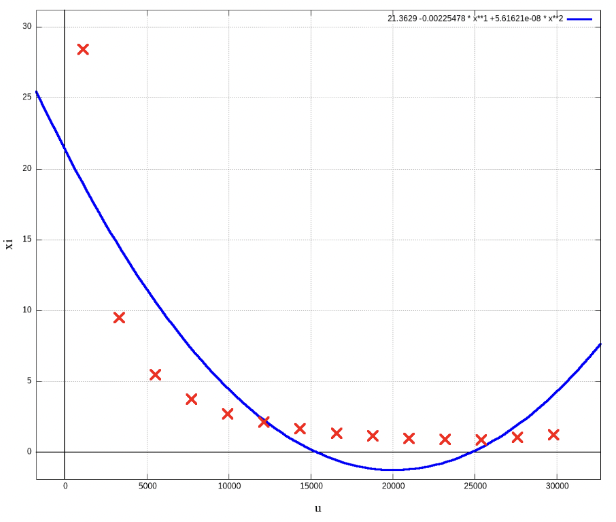
\includegraphics[width=0.8\textwidth]{4.png}
    \caption{график \( \xi(\nu) \)}
\end{figure}

Аппроксимируем прямой вида \( \psi = a\nu + b \) :
\[ a = 1.3\cdot 10^{-4} \pm 6.3\cdot 10^{-6} \]
\[ b = 4.55 \pm 0.06 \]

\begin{figure}[H]
    \centering
    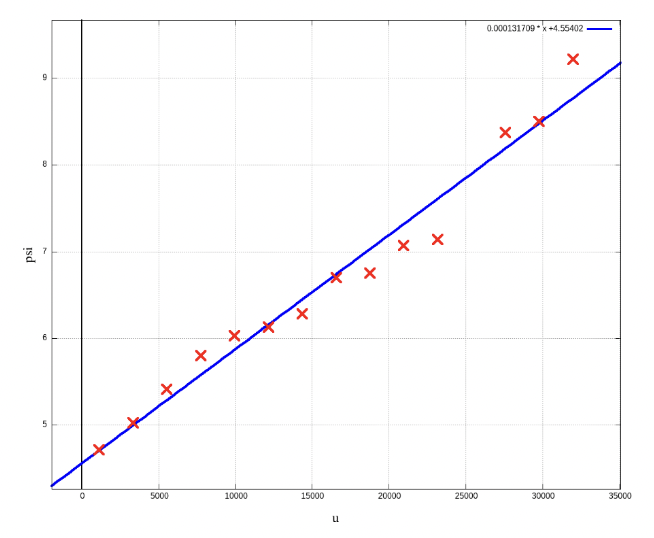
\includegraphics[width=0.8\textwidth]{5.png}
    \caption{график \( \psi(\nu) \)}
\end{figure}

\subsection{Зависимость \(L\) от \(\nu\)}

\begin{table}[H]
    \centering
    \begin{tabular}{|c|c|}
    \hline
    \(\nu\), Гц & \(L\), \(\mu H\) \\\hline
    40  & 550 \\\hline
    400 & 4300\\\hline
    750 & 3400\\\hline
    1000& 3200\\\hline
    1500& 3100\\\hline
    2000& 3060\\\hline
    2500& 3050\\\hline
    \end{tabular}
\end{table}

Аппроксимируем многочленом 2 степени:
\[ L = 4885 - 2.1\nu + 0.0006\nu^2 \]


\begin{figure}[H]
    \centering
    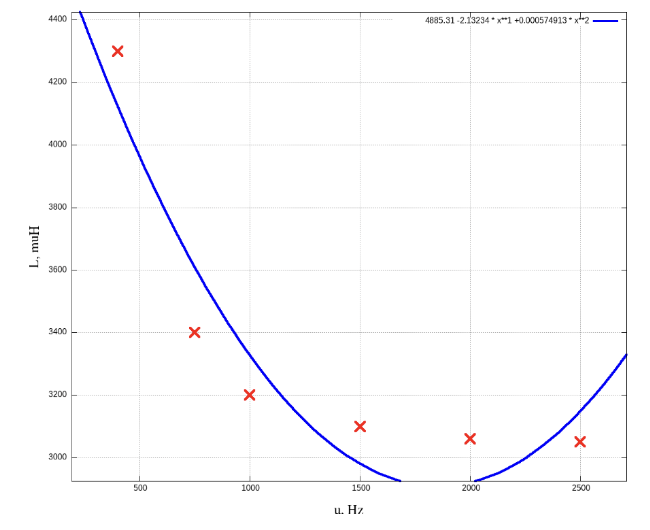
\includegraphics[width=0.8\textwidth]{6.png}
    \caption{график \( L(\nu) \)}
    \label{fig:L}
\end{figure}

\section {Обработка экспериментальных данных}
\subsection{}
\label{sigma_1}
По графикам на рисунках \ref{plot1} и \ref{plot2} легко убедиться что зависимость \( 1/\xi^2(\nu^2) \)
имеет линейный вид.

Экстраполируя полученную зависимость к точке \( \nu = 0 \), соответствующей величине \( \frac{|H_1|}{|H_0|} = 1 \)
определим коэффициент пропорциональности \( \xi_0 \) между \( \xi \) и \( \frac{|H_1|}{|H_0|} \): 
\[ \xi_0 = 53 \]

Из того что в области низких частот
\[ \left(\frac{|H_1|}{|H_0|}\right)^2 = (\xi_0\xi)^2 \simeq \frac{1}{1 + A\nu^2} \]
получим что угловой коэффициент зависимости \( 1/\xi^2(\nu^2) \) равен
\[ k = \pi ah\mu_0\xi_0\sigma = (0.096 \pm 7\cdot10^{-4}) \]
Отсюда найдём првоводимость меди:
\[ \sigma = \frac{k}{\pi ah\mu_0\xi_0} = 13.6\; \frac{МСм}{м} \]

\subsection\label{sigma_2}

Перерисуя график \( \psi \) от \( \nu \) и опроксимируя прямой получим:

\begin{figure}[H]
    \centering
    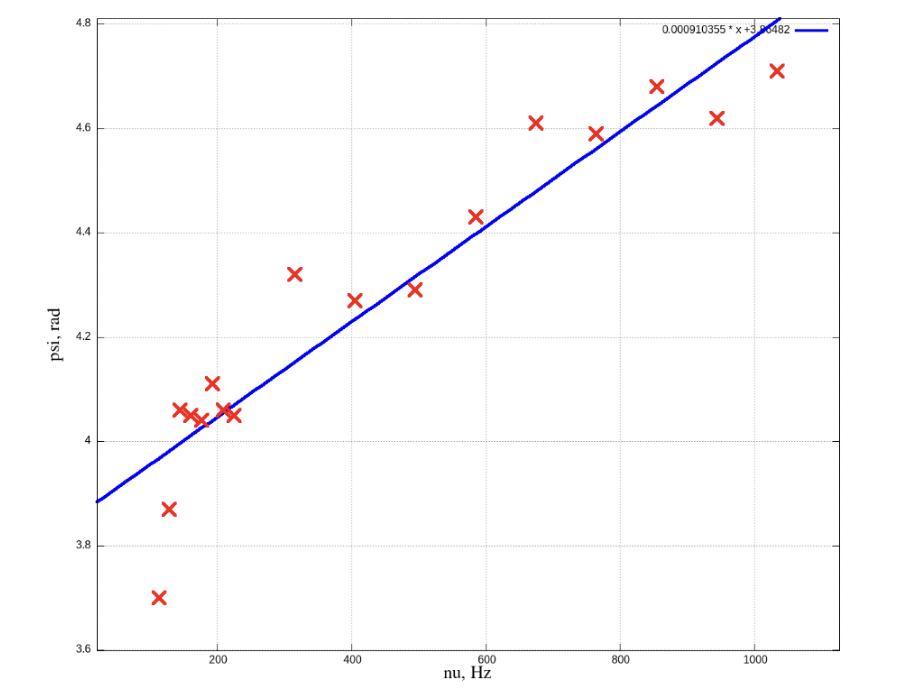
\includegraphics[width=0.8\textwidth]{psi.png}
    \caption{график \( \psi(\nu) \)}
\end{figure}

Полученная зависимость вида \( \psi = a\cdot\nu + b \)
\[ a = (9 \pm 0.08)\; 10^{-3} рад/Гц \]
\[ b = (3.9 \pm 0.02)\; рад \] 

Из того что 
\[ \tg(\psi) = \frac{ah}{\delta^2} \]
и
\[ \delta^2 = \sqrt{\frac{1}{\pi\nu\sigma\mu_0}} \]
получим:

\[ \tg(\psi) = \pi ah\sigma\mu_0\nu \]

И тогда через коэффицент пропорциональности в зависимости \( \psi(\nu) \) найдём проводимость меди:
\[ \sigma = \frac{\tg(\psi)/\nu}{\pi ah\mu_0} = 67.5\; \frac{МСм}{м} \]

\subsection{}\label{sigma_3}

Построим график зависимости \( \phi = \psi - \frac{\pi}{4} \) от \(\sqrt{\nu}\):

\begin{figure}[H]
    \centering
    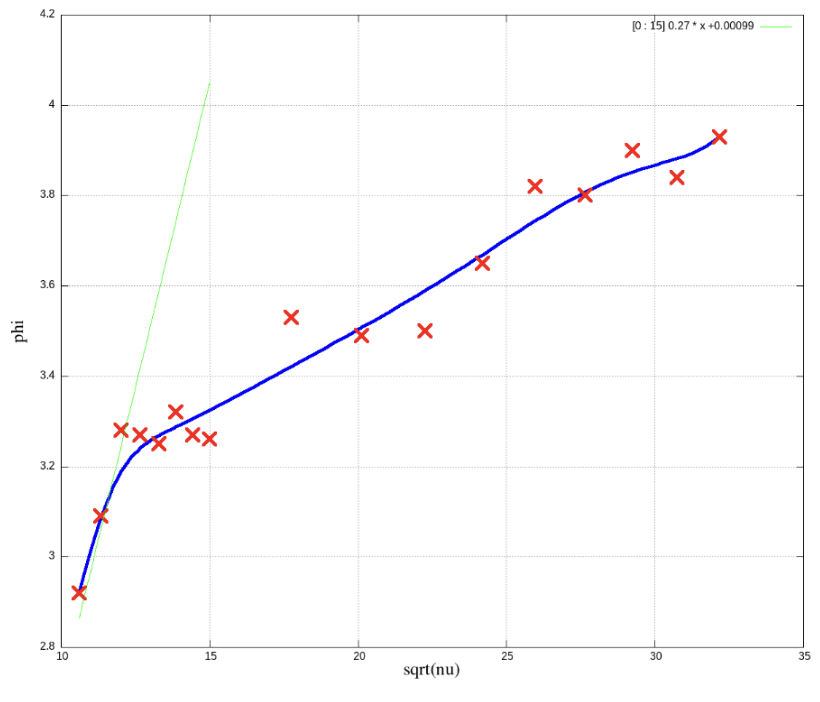
\includegraphics[width=0.8\textwidth]{phi.png}
    \caption{график \( \phi(\sqrt{\nu}) \)}
\end{figure}

Угловой коэффициент касательной:
\[ k = 0.27 \]

Отсюда, т.к.
\[ \psi = \frac{\pi}{4} + h\sqrt{\pi\nu\sigma\mu_0}\]
получим значение:
\[ \sigma = \frac{k^2}{h^2\pi\mu_0} = 8207\; \frac{МСм}{м}\]
Это значение не выглядит реалистичным, что можно связать с ошибками экспериментаторов во время
измерении разности фаз.

\subsection{} \label{sigma_4}
По результатам измерений, изображённым на Рис. \ref{fig:L} Определим максимальное и минимальное значение индуктивности:
\[ L_{min} = 550\; \mu H \]
\[ L_{max} = 3060\; \mu H \]

Построим график зависимости \( (L_{max} - L_{min})/(L - L_{min}) \) от \(\nu^2\) (\(10^6\; Гц^2\)):
\begin{figure}[H]
    \centering
    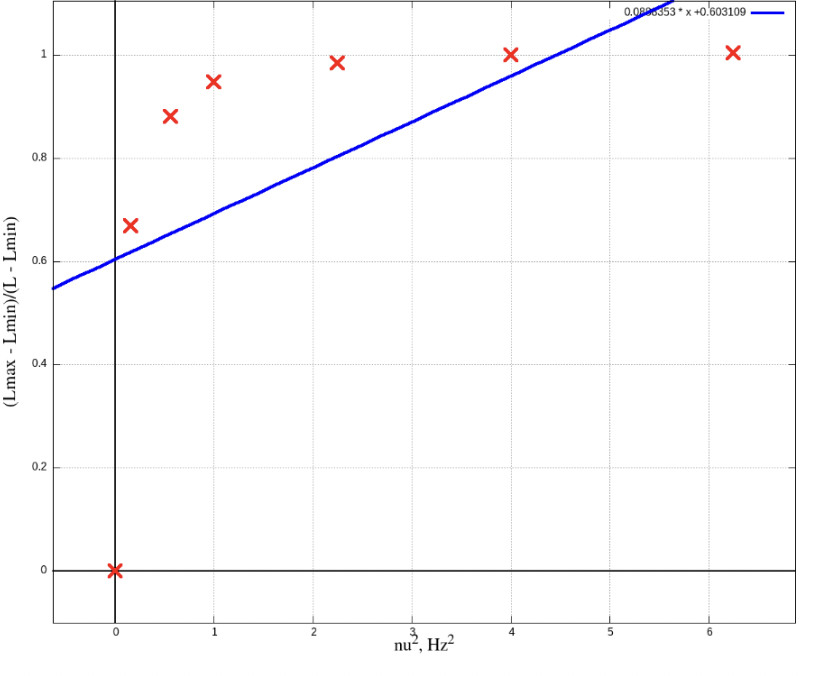
\includegraphics[width=0.8\textwidth]{L.png}
    \caption{график зависимости \( (L_{max} - L_{min})/(L - L_{min})\) от \(\nu^2 \cdot 10^6\; Гц^2\) \)}
\end{figure}

Из графика видно, что измерения плохо опроксимируются прямой. Скорее всего это произошло в виду
неправильного обращения экспериментаторов с измеряющим прибором и установкой. В следствии этого
оценить проводимость материала исходя из этого эксперимента не предоставляется возможным.

\subsection{}

Сравним значения проводимости медного экрана, полученные в ходе различных экспериментов:
\begin{table}[H]
    \centering
    \begin{tabular}{|c|c|c|c|c|}
        \hline
        \(\sigma\; 10^7 См/м\) из 3.1 & \(\sigma\; 10^7 См/м\) из 3.2  & \(\sigma\; 10^7 См/м\) из 3.3  & \(\sigma\; 10^7 См/м\) из 3.4&  \(\sigma\; 10^7 См/м\) табличное\\\hline
        1.36 & 6.75 & 820 & -- & 5.96  \\\hline
    \end{tabular}
\end{table}

Можно заметить, что значения полученные в пунктах 3.1 и 3.2 достаточно близки к табличному.
В то же время значение, полученное в пункте 3.3 далеко от табличного, а в 3.4 его вычисление
и вовсе не предоставляется возможным, что можно связать с ошибками экспериментаторов в ходе этих экспериментов.

\subsection{}
Расчитаем, используя значение \(\xi_0 = 53\), полученное в пункте 3.1, значение \(|H_1|/|H_0|\) для всех измерений.
Используем формулу
\[\frac{H_1}{H_0} = \xi\xi_0\]
(
Так же получим из формулы
\[ \frac{H_1}{H_0} = \frac{1}{\cosh(\alpha h) + \frac{1}{2}\alpha a\cdot\sinh(\alpha h)}, \]
где 
\[ \alpha = \sqrt{\2\pi\nu\sigma\mu}\cos(\pi/4) \]
а \(a\) и \(h\) - известные нам параметры установки, получим теоретические значения \(\frac{H_1}{H_0}\). 
Изобразим всё на графиках:

\begin{figure}[H]
    \centering
    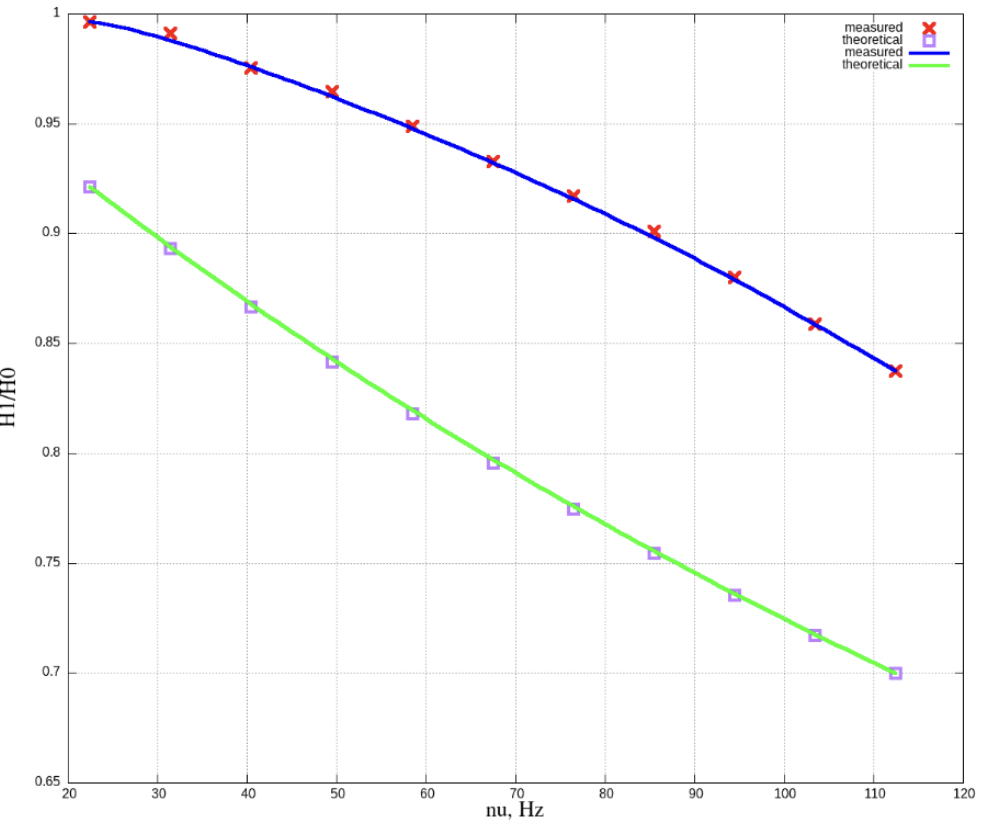
\includegraphics[width=0.8\textwidth]{H-low.png}
    \capture {Теоретический и экспериментальный графики зависимостей \(H_1/H_0\) от \(\nu\) для низких частот}
    \label{H-low}
\end{figure}

\begin{figure}[H]
    \centering
    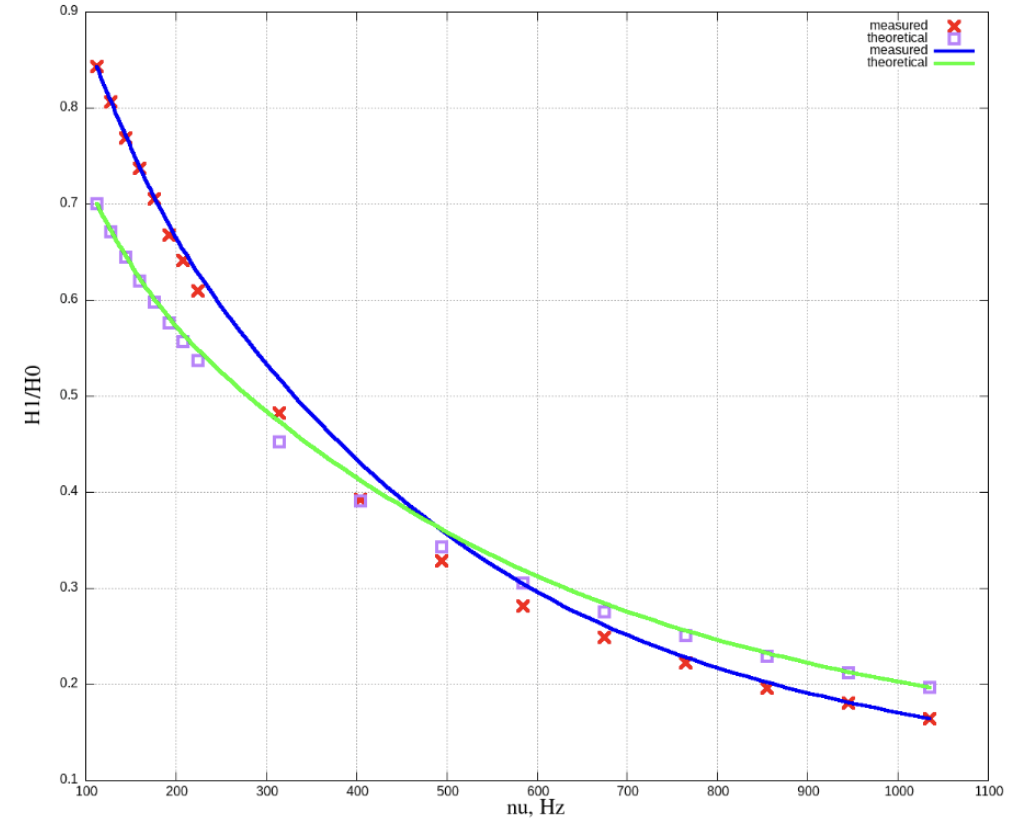
\includegraphics[width=0.8\textwidth]{H-mid.png}
    \capture {Теоретический и экспериментальный графики зависимостей \(H_1/H_0\) от \(\nu\) для средних частот}
    \label{H-mid}
\end{figure}

\begin{figure}[H]
    \centering
    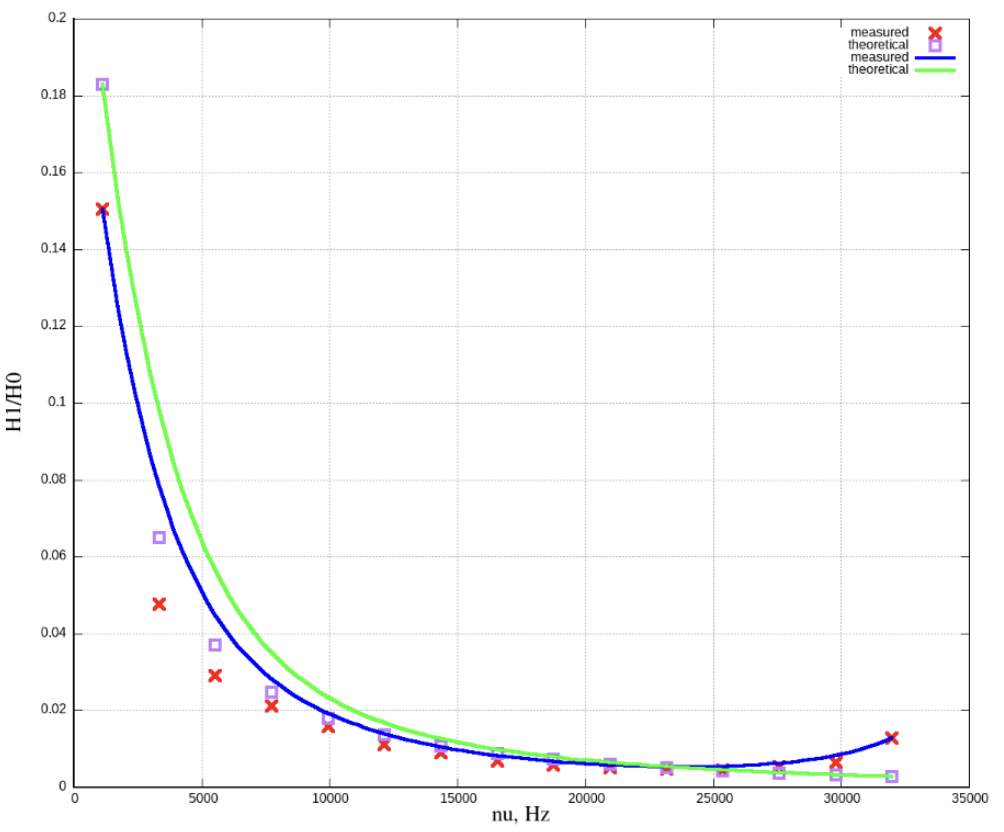
\includegraphics[width=0.8\textwidth]{H-hight.png}
    \capture {Теоретический и экспериментальный графики зависимостей \(H_1/H_0\) от \(\nu\) для высоких частот}
    \label{H-hight}
\end{figure}

Мы видим, что теоретические и экспериментальные значения \(H_1/H_0\) достаточно точно совпадают для всех диапазонов.
Наибольшее отличие заметно в области низких частот, что можно связать с недостаточной точностью вычислений или измерений в этом
диапазоне.


\section{Выводы}
Была проведена попытка измерения проводимости материала циллиндра 4 разными способами (теоретическое значение \( 5\cdot10^7\; \frac{См}{м} \)). Результаты:
\begin{enumerate}
    \item Из углового коэффициента зависимости \(1/\xi\) от \(\nu^2\). Получено значение \(1.36\cdot10^7\;\frac{См}{м}\). Это значение поп порядку
    совпадает с табличным.
    \item Из зависимости \( \tg(\psi) \) от \( \nu \). Получено значение \( 6.75\cdot10^7\; \frac{См}{м} \) . Это значение очень близко к табличному.
    \item Из угла наклона касательной к графику \( \psi \) от \(\sqrt{\nu}\) в области низких частот. Получено значение \( 821\cdot10^7\; \frac{См}{м} \),
    что отличается от табличного на несколько порядков.
    \item Из зависимости \( (L_{max} - L_{min})/(L - L_{min}) \) от \(\nu^2\). Попытка вычисления \(\sigma\) оказалась неудачной, т.к. измеренные значения
    нельзя хоть сколько-нибудь точно опроксимировать прямой.
\end{enumerate}
Можно сделать вывод, что только первые 2 способа измерения \(\sigma\) оказались удачными и дали правильные значения.

Были сравнены теоретически-вычисленное и измеренные значения отношения амплитуд магнитных полей для низких, средних и высоких частот.
Все сравнения показывают, что, хоть и в области низких частот значения незначительно отличались, тренд оказался одинаковым.

\end{document}